\begin{figure}[H]
	\caption{Diagram of the spaceship taking a linear path.}
	\label{fig:linearCase}
	\centering
	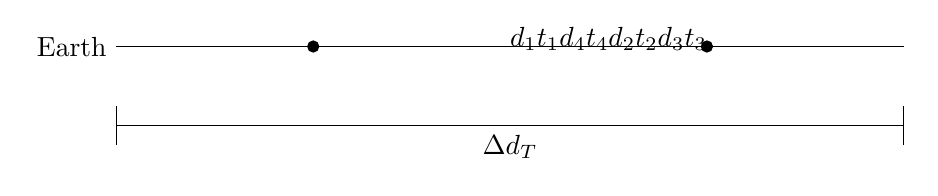
\begin{tikzpicture}
		\coordinate [label=left:Earth] (E) at (-5,0);
		\coordinate (N) at (5,0);
		\coordinate (M) at (0,0);
		\coordinate (Me) at (-2.5,0);
		\coordinate (Mn) at (2.5,0);

		\coordinate (TL) at (-5,-1);
		\coordinate (TR) at (5,-1);
		\coordinate [label=below:$\Delta d_T$](T) at (0,-1);

		\draw (E) -- (N);
		\draw (TL) -- (TR);
		\draw (-5,-0.75) -- (-5,-1.25);
		\draw (5,-0.75) -- (5,-1.25);

		\tkzLabelSegment[above=1em](E,Me){$\Del d_1$};
		\tkzLabelSegment[above](E,Me){$\Del t_1$};
		\tkzLabelSegment[above=1em](Me,M){$\Del d_4$};
		\tkzLabelSegment[above](Me,M){$\Del t_4$};

		\tkzLabelSegment[above=1em](M,Mn){$\Del d_2$};
		\tkzLabelSegment[above](M,Mn){$\Del t_2$};
		\tkzLabelSegment[above=1em](Mn,N){$\Del d_3$};
		\tkzLabelSegment[above](Mn,N){$\Del t_3$};

		\filldraw[black] (E) circle (2pt);
		\filldraw[black] (N) circle (2pt);
		\filldraw[black] (M) circle (2pt);
	\end{tikzpicture}
\end{figure}
